% The Mexican hat potential is one that elicits spontaneous symmetry breaking (SSB), a process by which a physical system starting in a symmetric state spontaneously enters and remains in an asymmetric state. This usually applies to systems whose equations of motion obey a set of symmetries while the lowest-energy state(s) do(es) not. When the system assumes one of its ground states, its symmetry is broken even though the Lagrangian as a whole retains it. https://wikipedia.org/wiki/Spontaneous_symmetry_breaking
% See https://tikz.netlify.app/higgs-potential for a very similar image.

\documentclass[svgnames]{standalone}
\usepackage{pgfplots}
\pgfplotsset{compat=1.8}
\usetikzlibrary{arrows.meta}

\begin{document}
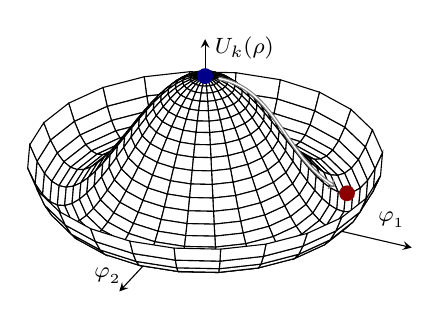
\begin{tikzpicture}[font=\footnotesize]
  \begin{axis}[
      axis lines=center,
      axis equal,
      domain=0:360,
      y domain=0:1.25,
      y axis line style=stealth-,
      y label style={at={(0.35,0.18)}},
      xmax=1.6,zmax=1.3,
      xlabel = $\varphi_{_1}$,
      ylabel=$\varphi_{_2}$,
      zlabel=$U_k(\rho)$,
      ticks=none
    ]
    \addplot3 [surf,shader=flat,draw=black,fill=white,z buffer=sort] ({sin(x)*y}, {cos(x)*y}, {(y^2-1)^2});
    \coordinate (center) at (axis cs:0,0,1);
    \coordinate (minimum) at (axis cs:{cos(30)},{sin(30)},0);
  \end{axis}

  \fill[DarkBlue] (center) circle (0.1);
  \fill[DarkRed] (minimum) circle (0.1);
  \draw (center) edge[shorten <=5,shorten >=5,out=-10,in=150,double,draw=gray,double distance=0.5,-{>[length=2,line width=0.5]}] (minimum);
\end{tikzpicture}
\end{document}
